\chapter{Selection}
\label{ref:selection}

This chapter describes the selection procedure for samples used in this
analysis which involves two parts: online and offline selection.
The first online selection are a composition of
pre-defined triggers and cuts provided by the LHCb experiment;
some of them may be limiting so extra care is needed to avoid biasing important
physical quantities.
The follow-up offline selection are entirely imposed by analysts
to further balance signal selection and background rejection efficiencies.

Most of the samples are directly used in building fit templates;
the selection procedure for these are discussed in \cref{ref:selection:data} and
\cref{ref:selection:mc}.
Selection of samples used in auxiliary studies is discussed in
\cref{ref:selection:aux-study}.


\section{Real data}
\label{ref:selection:data}

This analysis currently uses 1665~pb$^{-1}$ of proton-proton collision data
recorded by LHCb in 2016, at $\sqrt{s} = 13$~TeV.
It is planned to extend the use of data to 2016-2018 LHCb data.


\subsection{Signal data sample}

The \Dz\mun final states, henceforth referred as \Dz channel, are selected first
by an online trigger path,
a composition of hardware and fast software triggers,
listed in \cref{tab:triggers}.
%%%%
The L0 triggers are chosen to make sure events are not trigged by \muon
\emph{alone} which will introduce a \pt bias\footnote{
    According to table 1 in \cite{LHCb-DP-2019-001},
    the minimum \pt threshold across all L0 triggers is 1.35 GeV for 2018
    L0Muon trigger.
} on \muon,
which is very problematic for this analysis as \muon from signal
$\tauon \rightarrow \muon \neumb \neut$ decays are typically softer and
have smaller \pt,
making signal events less likely to be selected.
%%%%
The HLT1 paths are updated to the inclusive triggers for LHCb run 2,
as described in \cite{LHCb-INT-2019-025}, Section 6.7.1.
The \smalltt{Hlt2XcMuXForTauB2XcMu} is specifically designed for this analysis
to maintain minimal \pt bias on selected \muon.
The cuts imposed by the HLT2 line are listed in \cref{tab:cut-hlt2}.
%%%%
The \smalltt{Strippingb2D0MuXB2DMuForTauMuLine} requirements are
listed in \cref{tab:cut-stripping}.
Overall, the trigger path requires a \muon candidate to form a vertex with a
high $p_T$ $\Dz (\rightarrow \Km \pip)$ candidate, without any cut on the
invariant mass on the \Dz\mupm pair, nor on the \muon \pt.

\begin{table}[htb]
    \caption{Trigger path for this analysis.}
    \label{tab:triggers}
    \centering
    \parnotereset
    \begin{tabular}{c|c}
        \toprule
        {\bf Trigger level} & {\bf Requirements} \\
        \midrule
        L0 & \Dz L0Hadron TOS || \B L0Global TIS \\
        HLT1 & \makecell{
            (\kaon Hlt1TrackMVA TOS || \pion Hlt1TrackMVA TOS)\parnote{
                This is almost equivalent to \Dz Hlt1TrackMVA TOS, with a
                $\sim\!0.0027\%$ difference in selected events in
                reconstructed data sample in \Dz channel.
                Henceforth these two trigger paths are considered equivalent.
            } || \\ \Dz Hlt1TwoTrackMVA TOS
        } \\
        HLT2 & \B Hlt2XcMuXForTauB2XcMu \\
        \bottomrule
    \end{tabular}
    \begin{flushleft}
        \parnotes
    \end{flushleft}
\end{table}

\begin{table}[htb]
    \caption{Cuts defined in \smalltt{Hlt2XcMuXForTauB2XcMu}.}
    \label{tab:cut-hlt2}
    \centering
    \begin{tabular}{ c | rll}
        \toprule
        {\bf Particle} & {\bf Variable}               & {\bf Cuts}               \\
        \midrule
        \kaon, \pion   & \pt                          & $> 200$ MeV              \\
                       & Max \pt                      & $> 800$ MeV              \\
                       & \ptot                        & $> 5$ GeV                \\
                       & \ipChiSq                     & $> 9$                    \\
                       & \PID{$K$}                    & $> 2\;(K)$, $< 4\;(\pi)$ \\
        \midrule
        \Dz            & \pt                          & $> 2000$ MeV             \\
                       & $|\pi\;\pt|+|K\;\pt|$        & $> 2.5$ GeV              \\
                       & $m$                          & 1830--1910 MeV           \\
                       & \anyChiSq{vertex}/ndf        & $< 10$                   \\
                       & \anyChiSq{FD}                & $> 25$                   \\
                       & \DIRA                        & $> 0.999$                \\
                       & Child pair \DOCA             & $< 0.1$ mm               \\

        \midrule
        \muon          & \ipChiSq                     & $> 16$                   \\

        \midrule
        \Dz\muon       & \anyChiSq{vertex}/ndf        & $< 15$                   \\
                       & \anyChiSq{FD}                & $> 50$                   \\
                       & \DIRA                        & $> 0.999$                \\
                       & \DOCA                        & $< 0.5$ mm               \\
        \bottomrule
    \end{tabular}
\end{table}


\section{MC simulation}
\label{ref:selection:mc}


\section{Auxiliary samples}
\label{ref:selection:aux-study}


\section{Trigger and stripping}
\label{ref:selection:stripping}

The trigger paths selected for this analysis are listed in \cref{tab:triggers}.



\begin{table}[htb]
    \caption{Cuts defined in \smalltt{Strippingb2D0MuXB2DMuForTauMuLine}.}
    \label{tab:cut-stripping}
    \centering
    \begin{tabular}{c|rll}
        \toprule
        {\bf Event-Level }      & {\bf Variable}               & {\bf Cuts}               \\
        \midrule
        GEC                     & nSPDhits                     & $< 600$                  \\
        PV cut                  & nPV                          & $\geq1$                  \\
        \toprule
        {\bf Particle }         & {\bf Variable}               & {\bf Cuts}               \\
        \midrule
        $K, \pi$                & \pt                          & $> 300$ MeV              \\
                                & \ptot                        & $> 2$ GeV                \\
                                & \anyChiSq{IP}                & $> 9$                    \\
                                & \isMuon                      & \texttt{False}           \\
                                & \PID{$K$}                    & $> 4\;(K)$, $< 2\;(\pi)$ \\
                                & GhostProb                    & $< 0.5$                  \\
        \midrule
        \Dz                     & $|\pi\;\pt|+|K\;\pt|$        & $> 2.5$ GeV              \\
                                & $m - m_\text{PDG}$           & $< 80$ MeV               \\
                                & \anyChiSq{vertex}/nof        & $< 4$                    \\
                                & \anyChiSq{FD}                & $> 25$                   \\
                                & \DIRA                        & $> 0.999$                \\
        \midrule
        \muon                   & \ptot                        & $> 3$ GeV               \\
                                & \ipChiSq                     & $> 16$                  \\
                                & isMuon                       & \texttt{True}           \\
                                & \PID{$\mu$}                  & $> -200$                \\
                                & GhostProb                    & $< 0.5$                 \\
        \midrule
        \Dz\muon                & $m$                          & 0--10 GeV               \\
                                & \anyChiSq{vertex}/ndf        & $< 6$                   \\
                                & \DIRA                        & $>0.999$                \\
        \bottomrule
    \end{tabular}
\end{table}


\section{Candidate reconstruction}
\label{ref:selection:cand-reco}

Both real data and MC samples are reconstructed with \davinci{v45r6}.
For real data, only events passing corresponding stripping requirements are
reconstructed.
Due to the lack of stripping and minimal filtering for the MC samples, the
stripping selections (\cref{tab:cut-stripping}) are re-applied in \davinci,
without PID requirements.

The reconstruction sequences\footnote{
    The \davinci reconstruction script can be found at
    \techurllink{https://github.com/umd-lhcb/lhcb-ntuples-gen/blob/master/run2-rdx/reco_Dst_D0.py}{
        github/umd-lhcb/lhcb-ntuples-gen}.
}
are identical for both \Dz and \Dstar channels,
up to the reconstruction of \Dz\muon pair.
The \Dstar channel additionally requires a slow \pion\footnote{
    For real data, it is from the \texttt{StdAllLoosePions} TES location.
    For MC, \texttt{StdAllNoPIDsPions}.
} to form a \Dstar vertex with already reconstructed \Dz
which subsequently forms a \Bz vertex with reconstructed \muon.

Due to the fact that \Dstar\muon pairs arises from \Dz\muon pairs, as required
by the reconstruction sequences, some candidates will appear in both
\Dz and \Dstar channel, making the two channels correlated.
This correlation is removed by vetoing \Dstar candidates in the \Dz channel;
such procedure makes the two channels orthogonal, and is discussed in
\cref{ref:selection:veto}.


\section{Offline selections}
\label{ref:selection:offline}

Additional offline selections with stricter vertex quality and PID requirements,
mostly aligned with the old stripping line with the same name in LHCb run 1,
are applied to reconstructed samples.
The initial motivation was to bring 2016 data on par with run 1 data so
distributions of the same variables in 2016 and run 1 can be compared in a more
meaningful way,
providing check points for the development of this analysis.
Later, it is checked with a figure of merit study that the run 1 selections
are still optimal.
% TODO: Cite Alex's candidacy paper maybe?

The selections that are shared among \Dz and \Dstar channels are listed in
\cref{tab:offline-cut-common}.
The additional \Dz only selections are listed in \cref{tab:offline-cut-d0},
The \Dstar in \cref{tab:offline-cut-dst}.
Some of the selection variables are not standard LHCb variables;
these are marked in the tables and will be discussed in the subsequent sections.

\begin{table}[htb]
    \caption{Offline selections shared among \Dz and \Dstar channels.}
    \label{tab:offline-cut-common}
    \centering
    \begin{tabular}{c|rll}
        \toprule
        {\bf Event-Level }  & {\bf Variable}               & {\bf Cuts}               \\
        \midrule
        GEC                 & nSPDhits                     & $< 450$\parnote{
            This is to reduce correlation for \emph{TIS and TOS} candidates to make
            trigger emulation more robust.
            See \cref{ref:emulation-for-to-mc:correlation-tos-tis} for more details.
        }                                                                             \\
        \toprule
        {\bf Particle}      & {\bf Variable}               & {\bf Cuts}               \\
        \midrule
        $K, \pi$            & \pt                          & $> 500$ MeV              \\
                            & HLT1 TOS track \pt           & $> 1.7$ GeV              \\
                            & \ptot                        & $< 200$ GeV\parnote{
                                This is to make \ptot consistent with extended
                                \pidcalib binning.
                            }                                                         \\
                            & \anyChiSq{IP}                & $> 45$                   \\
                            & \isMuon                      & \texttt{False}           \\
                            & \PID{$K$}                    & $> 4\;(K)$, $< 2\;(\pi)$ \\
                            & GhostProb                    & $< 0.5$                  \\
        \midrule
        \Dz                 & \pt                          & $> 2$ GeV                \\
                            & $|\pi\;\pt|+|K\;\pt|$        & $> 1.4$ GeV              \\
                            & $\log(\IP)$\parnote{
                                \IP in terms of the \PrmVtx.
                                That is, the reconstructed \Dz is inconsistent
                                of coming from \PrmVtx directly.
                            }                              & $> -3.5$                 \\
                            & \anyChiSq{IP}                & $> 9$                    \\
                            & \anyChiSq{vertex}/ndf        & $< 4$                    \\
                            & \anyChiSq{FD}                & $> 250$                  \\
                            & \DIRA                        & $> 0.9998$               \\
        \midrule
        \muon               & \ptot                        & 3-100 GeV                \\
                            & $\log_{10}(1 - \vec{p}_\mu \cdot \vec{p}_i / (|p_\mu||p_i|))$,
                              $i \in \{K, \pi\}$
                                                           & $> -6.5$                 \\
                            & $\eta$                       & 1.7--5                   \\
                            & \ipChiSq                     & $> 45$                   \\
                            & GhostProb                    & $< 0.5$                  \\
                            & \PID{$\mu$}                  & $> 2$                    \\
                            & \PID{$e$}                    & $< 1$                    \\
                            & \UBDT\parnote{
                                This is a BDT-based \muon PID algorithm,
                                which is discussed in \cref{ref:selection:mu-pid}.
                            }
                                                           & $> 0.25$                 \\
        \bottomrule
    \end{tabular}
    \begin{flushleft}
        \parnotes
    \end{flushleft}
\end{table}

\begin{table}[htb]
    \caption{Offline selections exclusive to \Dz channel.}
    \label{tab:offline-cut-d0}
    \centering
    \begin{tabular}{c|rll}
        \toprule
        {\bf Particle}  & {\bf Variable}               & {\bf Cuts}      \\
        \midrule
        \Dz\muon        & $m$                          & $< 5200$ MeV    \\
                        & {\footnotesize$\begin{aligned}
                                \text{Max}(
                                    &|\Delta m_\text{veto,1} - 145.454|, \\
                                    &|\Delta m_\text{veto,2} - 145.454|
                                )
                           \end{aligned}$}\parnote{
                            \label{parnote:dst-veto}
                            To reduce overlapping events between
                            \Dz and \Dstar channels.
                            Discussed in \cref{ref:selection:veto}.
                        }                              & $> 4$ MeV       \\
                        & $\Delta m_\text{alt hypo}$\parnoteref{parnote:dst-veto}
                                                       & $> 165$ MeV     \\
                        & transverse flight distance   & $< 7$ mm        \\
                        & \anyChiSq{vertex}/ndf        & $< 6$           \\
                        & \DIRA                        & $> 0.9995$      \\
        \bottomrule
    \end{tabular}
    \begin{flushleft}
        \parnotes
    \end{flushleft}
\end{table}

\begin{table}[htb]
    \caption{Offline selections exclusive to \Dstar channel.}
    \label{tab:offline-cut-dst}
    \centering
    \begin{tabular}{c|rll}
        \toprule
        {\bf Particle}  & {\bf Variable}                 & {\bf Cuts}    \\
        \midrule
        slow \pion     & GhostProb                       & $< 0.25$      \\
        \midrule
        \Dstarp        & $|m - m_\Dz - 145.454|$\parnote{
                           This is to require $m_\Dstarp$ to close to
                           its PDG mass,
                           up to a reconstruction effect on
                           $m_\Dz$.
                       }                                 & $< 2$ MeV     \\
                       & \anyChiSq{vertex}/ndf           & $< 10$        \\
        \midrule
        \Dz\muon\parnote{
            This pair is not available at \davinci output.
        }              & \anyChiSq{vertex}/ndf \parnote{
                           This is extracted by
                           \texttt{TupleToolTagDiscardDstMu}.
                           Add this tool to the reconstructed \Bz
                           in \davinci.
                           The tool can be found at
                           \techurllink{https://github.com/umd-lhcb/TupleToolSemiLeptonic/blob/master/Phys/TupleToolSemiLeptonic/src/TupleToolTagDiscardDstMu.cpp}{
                               github/umd-lhcb/TupleToolSemiLeptonic
                           }.
                       }                                 & $< 6$         \\
                       & \DIRA\parnote{
                           This cut is applied at \davinci level,
                           \emph{not} offline.
                       }                                 & $> 0.999$     \\
        \midrule
        \Dstarp\muon   & $m$                             & $< 5280$ MeV  \\
                       & transverse flight distance      & $< 7$ mm      \\
                       & \anyChiSq{vertex}/ndf           & $< 6$         \\
                       & \anyChiSq{vertex}               & $< 24$        \\
                       & \DIRA                           & $> 0.9995$    \\
        \bottomrule
    \end{tabular}
    \begin{flushleft}
        \parnotes
    \end{flushleft}
\end{table}


\section{Muon PID}
\label{ref:selection:mu-pid}

It is reported from previous analyses
(\cite{PhysRevLett.115.111803,LHCb-ANA-2020-056}) that a tighter \muon PID
requirement was very helpful in reducing \muon misidentification
backgrounds\footnote{
    This means a charged particle of other species is misidentified as a \muon.
    For more details, see
    \cref{ref:data-driven-templates:mu-misid:unfold-fake-mu}.
}.
To maintain minimum bias on \muon \pt, a multivariate BDT,
referred as \UBDT, using uBDT method in TMVA class,
is trained to reject misidentified \muon while keeping rejection
efficiency flat on \pt,
as described in \cite{LHCb-ANA-2020-056}.

The \UBDT has been re-trained on LHCb run 2 MC\footnote{
    The updated project can be found at
    \techurllink{https://github.com/umd-lhcb/MuonBDTPid}{github/umd-lhcb/MuonBDTPid}.
}.
There is ongoing effort to study its efficiency against standard run 2 PID
variables.
Early report suggests the flatness on \pt is maintained while rejection
efficiencies relative to existing PID cut are high for all but proton ($p$),
as shown in \cref{fig:ubdt-eff}.

% Generated with:
%   https://github.com/umd-lhcb/pidcalib2, branch efficiency_study
% first, run efficiency_gen/rdx-run2-ubdt-misidgen.sh
% then, go inside scripts folder, run ./plots.py
\begin{figure}[htb]
    \centering
    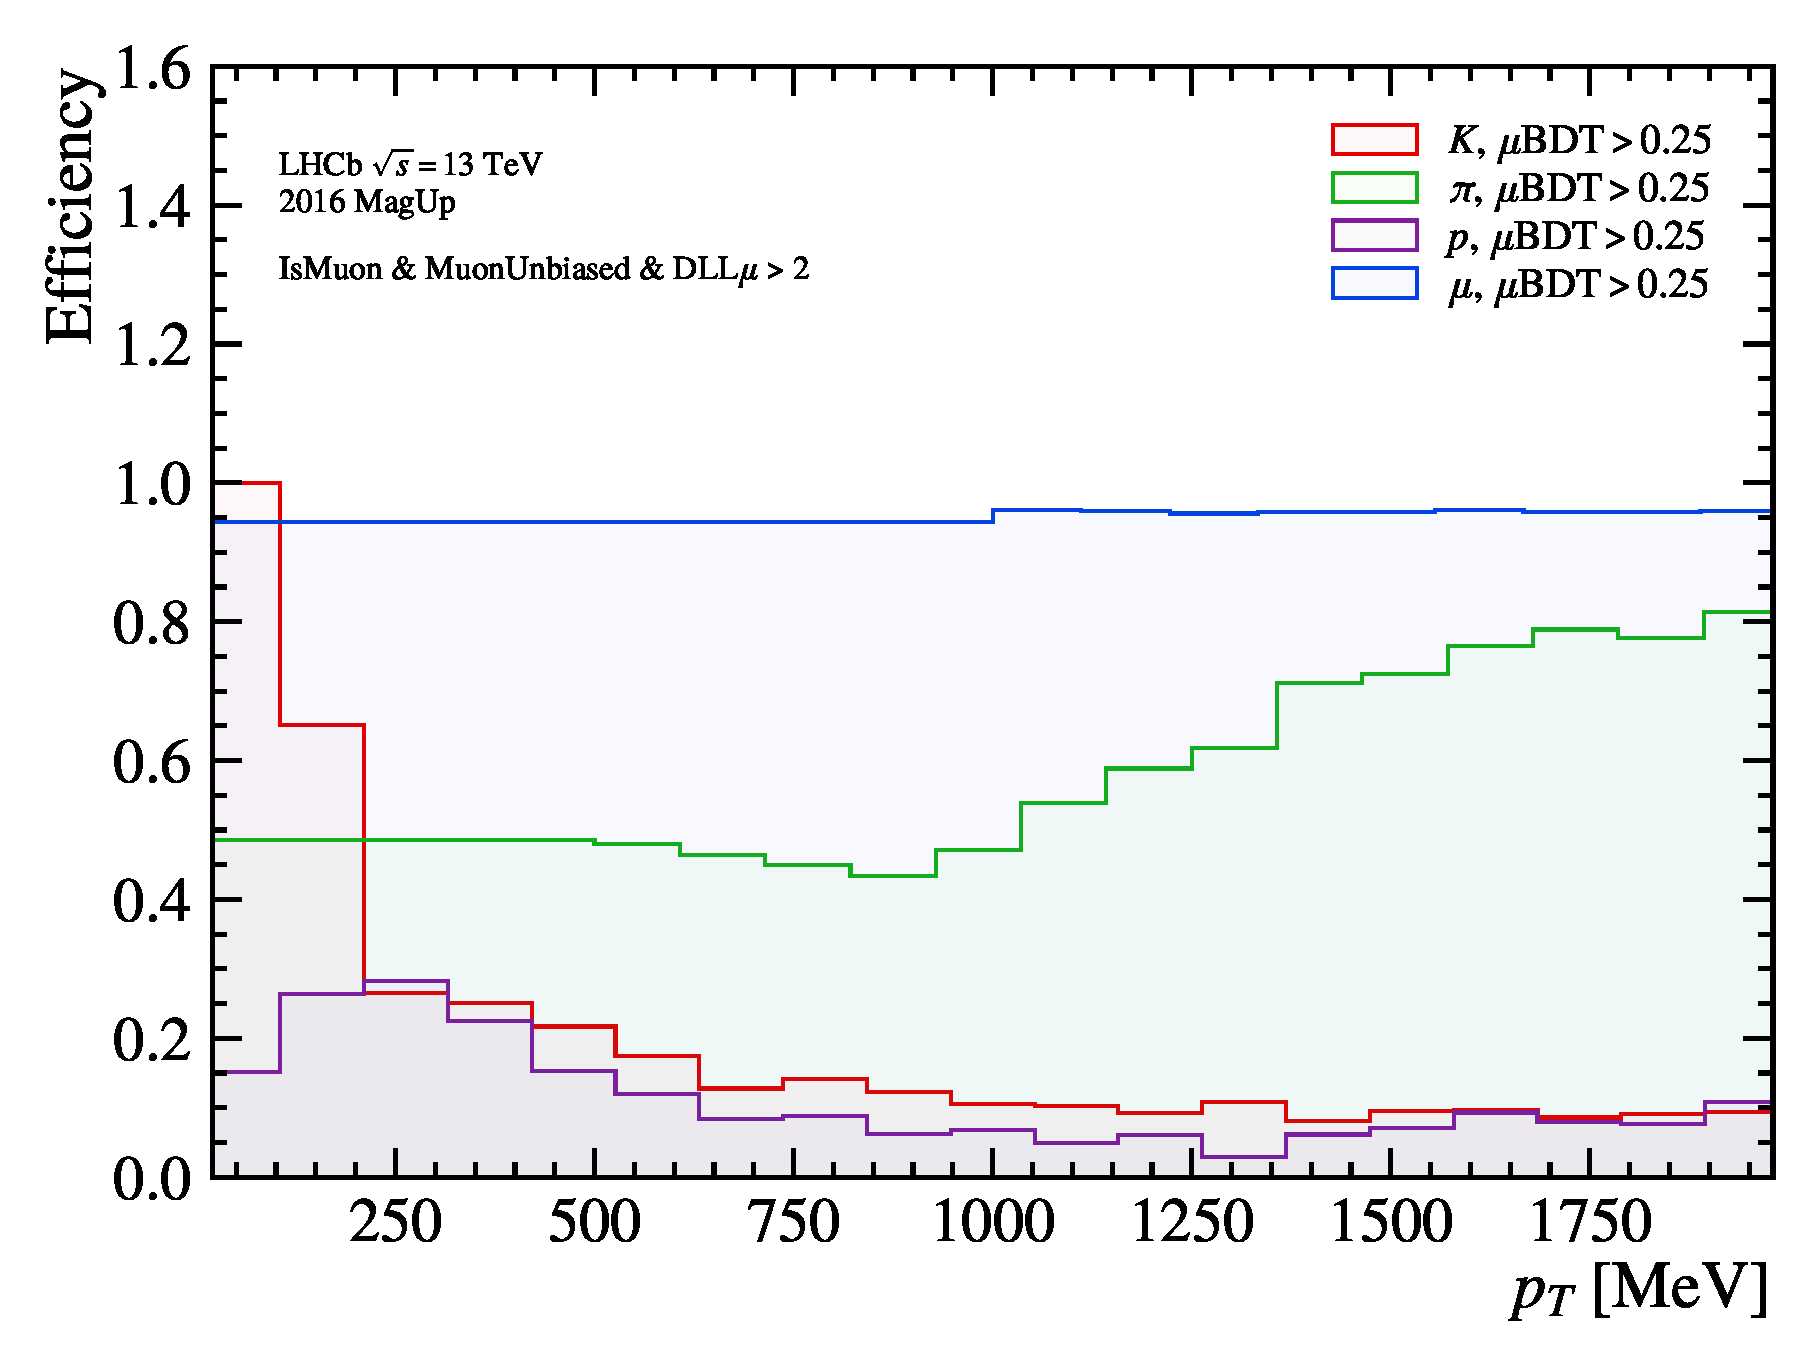
\includegraphics[width=0.45\textwidth]{./figs-selection/eff_Brunel_PT_up_pidcalib_ubdt_eff.pdf}
    \hspace{1em}
    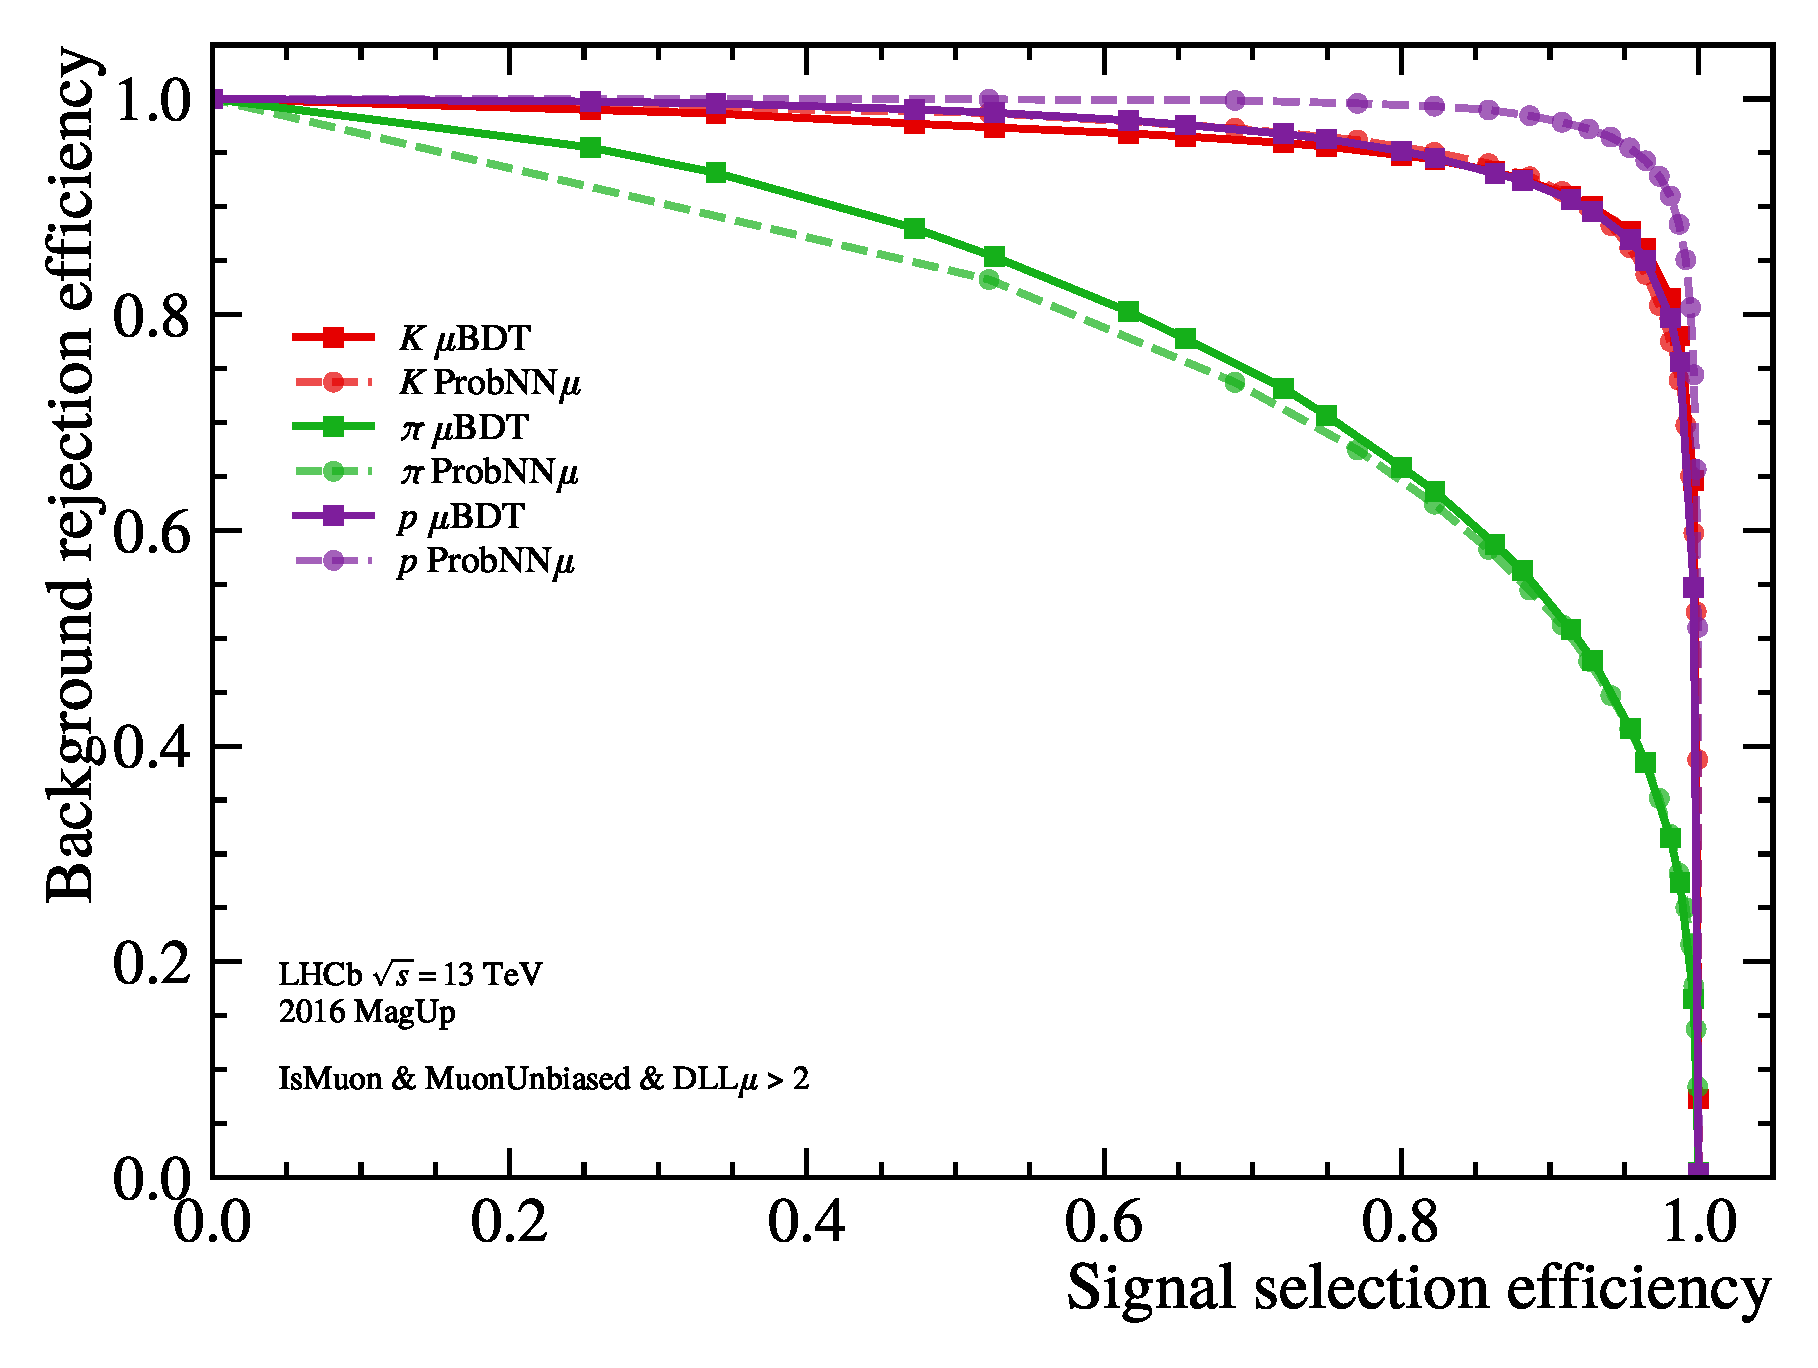
\includegraphics[width=0.45\textwidth]{./figs-selection/rej_v_eff_unbiased_Brunel_PT.pdf}

    \caption{
        Preliminary \UBDT study.
        Left: \UBDT \muon selection efficiency is flat in \pt, with
        global cut \isMuon \& $\text{\PID{\muon}}\! > 2$,
        and $\UBDT > 0.25$.
        Right: with the same global cut, \UBDT is more effective in rejecting
        \pion than LHCb official \ProbNN{\muon}.
        The \kaon rejection efficiencies are similar between the two;
        the $p$ rejection efficiency is lower for \UBDT, but the absolute
        rejection efficiency is high enough.
    }
    \label{fig:ubdt-eff}
\end{figure}


\section{Selected signal (ISO) and control (1OS, 2OS, DD) samples}
\label{ref:selection:skims}

The signal and control samples are selected by inspecting if there exists
additional charged tracks that are compatible with coming from the
reconstructed \B vertex.
To predict the possibility of a charged track originating from the \B vertex,
a multivariate BDT, referred as ``isolation BDT'', is used.
The BDT is conceptually identical to the one used in
\cite{LHCb-ANA-2020-056} but with the BDT re-trained based on LHCb run 2
simulation.

The isolation BDT\footnote{
    The isolation BDT can be found at
    \techurllink{https://github.com/umd-lhcb/TupleToolSemiLeptonic/blob/master/Phys/TupleToolSemiLeptonic/src/TupleToolApplyIsolation.cpp}{github/umd-lhcb/TupleToolSemiLeptonic}.
} is added to the \davinci reconstruction sequence.
It loops over all charged tracks in the event\footnote{
    More specifically, these tracks are coming from
    \texttt{StdAllNoPIDsPions}, \texttt{StdNoPIDsUpPions},
    and \texttt{StdNoPIDsVeloPions}.
},
providing isolation scores for each of them where
higher score implies higher probability of coming from the vertex, named as
``anti-isolated''.
Three tracks with highest isolation scores\footnote{
    The ones that are most likely to be anti-isolated.
} are saved in the output file, in descending order\footnote{
    So the first one is the most anti-isolated one among all charged tracks
    in the event.
}.

Below a brief description for the signal sample and the main physics background
control samples is provided.
The actual isolation selections are listed in \cref{tab:skim-cut}.

\begin{itemize}
    \item ISO: $B \rightarrow D^{(*)} \lepton \neulb$, with $\lepton \in \{\muon,
        \tauon\}$.
        This is referred as signal, or ``isolated'', sample.
        It requires that no additional charged track is from the \B vertex
        (in a probabilistic sense, with probability related to the isolation
        score)
        and is compatible with a fully reconstructed \B decay
        (ignoring missing neutrino(s)).

    \item DD: $B \rightarrow D^{(*)}D X$,
        with dominate $D \rightarrow \Kp \mun \neumb X$ sub-decays.
        This is a double-charm ($DD$) control sample,
        which is selected by requiring at least one anti-isolated track,
        a \kaon-like long track\footnote{
            This means the track went through both upstream and downstream
            trackers, and is generally of good tracking quality.
        } and a hard track in the three most anti-isolated tracks\footnote{
            Note that these three requirements can be satisfied by a single
            track.
        }.

    \item 1OS: $B \rightarrow D^{**} \lepton \neulb$.
        This control sample, enriched in excited charm states,
        requires one and only one additional anti-isolated charged long track
        that is compatible with a \pion PID hypothesis and has correct charge
        for a $D^{**} \rightarrow D^{(*+)}\pim$ decay.

    \item 2OS: $B \rightarrow D^{**}_H \lepton \neulb$,
        where $H$ stands for ``heavy''.
        This control sample is enriched in highly excited (heavy) charm states,
        which is selected by requiring two and only two anti-isolated \pion-like
        long tracks of opposite charge,
        capable of $D^{**}_H \rightarrow D^{(*)} \pip\pim$ decay.

        % Why?
        This sample also provides an independent selection of
        $B \rightarrow D^{(*)}D X$ backgrounds, where the \pip\pim fit into the
        $X$ category and \kaon escapes isolation detection.
\end{itemize}

\begin{table}[htb]
    \caption{Signal and control sample isolation requirements.}
    \label{tab:skim-cut}
    \centering
    \begin{tabular}{c|rll}
        \toprule
        {\bf Sample}  & {\bf Variable}              & {\bf Cuts}     \\
        \midrule
        ISO           & \isoBDT{1}                  & $< 0.15$       \\
        \midrule
        1OS           & \isoBDT{1}                  & $> 0.15$       \\
                      & \isoBDT{2}                  & $< 0.15$       \\
                      & \isoTrack{1}                & $= 3$\parnote{
                          This means a long track.
                      }                                              \\
                      & $p_1$                       & $> 5$ GeV      \\
                      & $p_{T,1}$                   & $> 0.15$ GeV   \\
                      & \ProbNN{$K_1$}              & $< 0.2$        \\
                      & $Q_1 \cdot \text{PID}_\Dz$\parnote{
                          Apply to \Dz channel,
                          which implies that the anti-isolated \pip can
                          form a \Dstarp with the \Dz.
                      }                             & $> 0$          \\
                      & $Q_1 \cdot \text{PID}_\Dstar$\parnote{
                          Apply to \Dstar channel.
                          Here it is required that the anti-isolated \pim can
                          form a $D^{**0}$ with the \Dstarp.
                      }                             & $< 0$          \\
        \midrule
        2OS           & \isoBDT{1}                  & $> 0.15$       \\
                      & \isoBDT{2}                  & $> 0.15$       \\
                      & \isoBDT{3}                  & $< 0.15$       \\
                      & \isoTrack{1}                & $= 3$          \\
                      & \isoTrack{2}                & $= 3$          \\
                      & {\footnotesize
                         Max$(p_1 \cdot (p_{T,1} > 0.15 \text{ GeV}),
                              p_2 \cdot (p_{T,2} > 0.15 \text{ GeV}))$
                        }
                                                    & $> 5$ GeV      \\
                      & \ProbNN{$K_1$}              & $< 0.2$        \\
                      & \ProbNN{$K_2$}              & $< 0.2$        \\
                      & $Q_1 \cdot Q_2$             & $< 0$          \\
        \midrule
        DD            & \isoBDT{1}                  & $> 0.15$       \\
                      & {\footnotesize$\begin{aligned}
                            \text{Max}(
                            &p_1 \cdot (p_{T,1} > 0.15\text{ GeV}),  \\
                            &p_2 \cdot (p_{T,2} > 0.15\text{ GeV})
                                 \cdot (\text{\isoBDT{2}} > -1.1),   \\
                            &p_3 \cdot (p_{T,3} > 0.15\text{ GeV})
                                 \cdot (\text{\isoBDT{3}} > -1.1)
                            )
                        \end{aligned}$}             & $> 5$ GeV      \\
                      & Max(\ProbNN{$K_{1,2,3}$})   & $> 0.2$        \\
                      & \isoTrack{\text{the one passing $K$ PID requirement}}
                                                    & $= 3$          \\
                      & \isoBDT{\text{the one passing $K$ PID requirement}}
                                                    & $> -1.1$       \\
        \bottomrule
    \end{tabular}
    \begin{flushleft}
        \parnotes
    \end{flushleft}
\end{table}


\section{Veto of overlapping candidates}
\label{ref:selection:veto}

% See this note: https://github.com/umd-lhcb/rdx-run2-analysis/blob/master/docs/cuts/Dst_veto_in_D0.md
% TODO: The number need to be updated
Since the reconstruction of a \Dstar\muon pair always requires the existence
of a \Dz\muon pair,
there is about 35\% of events in the signal sample of the \Dstar
channel leaks into \Dz channel.
This is likely due to the fact that slow \pion typically has poor tracking
resolution (small \ipChiSq), making the \Dz\pion vertex of poor quality which
makes the reconstruction fail and \Dstar partially reconstructed as \Dz.

To veto the overlapping candidates between \Dz and \Dstar channel,
a tool\footnote{
    Named \texttt{TupleToolApplyIsolationVetoDst}, which can be found at
    \techurllink{https://github.com/umd-lhcb/TupleToolSemiLeptonic/blob/master/Phys/TupleToolSemiLeptonic/src/TupleToolApplyIsolationVetoDst.cpp}{github/umd-lhcb/TupleToolSemiLeptonic}
}.
is added to the \davinci reconstruction sequence, which processes all tracks
in the event with the following procedure:

\begin{enumerate}
    \item Denote the track as $t$
    \item Refit a vertex from \Dz and $t$.
    \item Compute $\Delta m_\text{veto} \equiv m_{\Dz t} - m_\Dz$
    \item Test if $\Delta m_\text{veto} \in [140~\text{GeV}, 160~\text{GeV}]$.
        If it is, record $\Delta m_\text{veto}$ and the isolation BDT
        score of this track.
\end{enumerate}

From all recorded BDT scores and $\Delta m_\text{veto}$, the
$\Delta m_\text{veto}$ of the tracks with top two BDT scores are saved.
It is then filtered offline (listed in \cref{tab:offline-cut-d0})
that these two tracks,
the best slow \pion candidates,
are \emph{incompatible} with
forming a \Dz\pion vertex with a mass close to \Dstar PDG mass.

Note that this tool does not rank tracks based \emph{solely} on the isolation,
because the poor tracking resolution of the slow \pion implies that the track is
\emph{not guaranteed} to have a large isolation score, as it maybe more
compatible to be originating from PV, instead of the \B vertex.
Ranking tracks that fall within the $[140~\text{GeV}, 160~\text{GeV}]$
mass window based on their BDT scores
makes the veto procedure more robust, as reported in \cite{LHCb-ANA-2020-056}.

In addition, an alternative mass hypothesis is tested
(offline, also listed in \cref{tab:offline-cut-d0}), where the reconstructed
\muon is treated as a \pion,
and $\Delta m_\text{alt hypo} = m_{\Dz\muon_\text{as \pion}} - m_\Dz$
is computed\footnote{
    By using the 3-momentum of the \muon, while using $m_\pion$ as the invariant
    mass of the track.
} and required to be inconsistent with \Dstar PDG mass.

The veto procedures are applied on all samples of the \Dz channel only.
